\documentclass[headsepline=true, abstracton]{scrartcl}

\usepackage[utf8]{inputenc}
\usepackage[T1]{fontenc}

\usepackage{amssymb}
\usepackage{amsmath}
\usepackage{amsthm}
\usepackage{bm}

\usepackage{natbib}

\usepackage[table,xcdraw]{xcolor}

\usepackage{graphicx}

\usepackage{geometry}
\usepackage{float}

\usepackage{setspace}

\usepackage{url}
 
 
 
  
\begin{document}



\renewcommand{\refname}{Bibliography}


\onehalfspacing
\setlength{\headsep}{15mm}


\thispagestyle{plain}

\title{\Large \textbf{Appendix:} \\ Generative Dynamics of Supreme Court Citations: \\ Analysis with a New Statistical Model}
%\author{}
 % Toggle % below to blind and unblind the manuscript
%  \author[1]{Christian Schmid \thanks{cxs5700@psu.edu}}
%   \author[2]{Ted Hsuan Yun Chen\thanks{thc126@psu.edu}}
% \author[2]{Bruce A. Desmarais\thanks{bdesmarais@psu.edu}}
% \author[1]{David R. Hunter \thanks{dhunter@stat.psu.edu}}
% \affil[2]{Department of Political Science, Pennsylvania State University}
 %\affil[1]{Department of Statistics, Pennsylvania State University}

\author{%
  Christian S. Schmid\footnote{Department of Statistics, The Pennsylvania State University, schmid@psu.edu}%
  \and Ted Hsuan Yun Chen \footnote{Department of Political Science, The Pennsylvania State University, thc126@psu.edu}%
   \and Bruce A. Desmarais \footnote{Department of Political Science, The Pennsylvania State University, bdesmarais@psu.edu}%
  \and David R. Hunter \footnote{Department of Statistics, The Pennsylvania State University, dhunter@stata.psu.edu}%
  }


\maketitle

\section{Goodness-of-Fit}
We evaluate the goodness-of-fit of the model following \citet{hunter2008goodness} by examining the distribution of four hyper statistics, e.g., the out- and indegree distribution and the distribution for two different edgewise shared partners statistics. OTP stands for \textit{outgoing two-paths} and refers to the number of cases $r$ that are cited by case $i$ and that cite case $j$, while $j$ is also directly cited by $i$. The second ESP statistic is the OSP specification that has been introduced in section 4.1.2 in the paper. Figure \ref{GOF} visualizes the goodness-of-fit results for the citation network for the 1950 (top) and 2015 (bottom) term. The solid black line indicates the statistic's distribution in the Supreme Court citation network of that given term and the boxplots depict the statistic's distribution of $1000$ networks that have been simulated from the ERGM defined by the MCMLE. This means that in the ideal case the solid black line passes through ever single boxplot.


We see that our models do a good job capturing the out and indegree distribution of the citation network, since the black line falls almost exclusively within the ranges spanned by the boxplots. For the ESP distributions we can observe that the number of ties with $r=0$ shared partners is captured well for both the OTP as well as for the OSP statistic. However, the model overestimates the number of $r=1$ shared partners and then, especially in the 2015 term network, underestimates the number of ties with more than $r=1$ shared partners. 

 \begin{figure}[H]
 \begin{center}
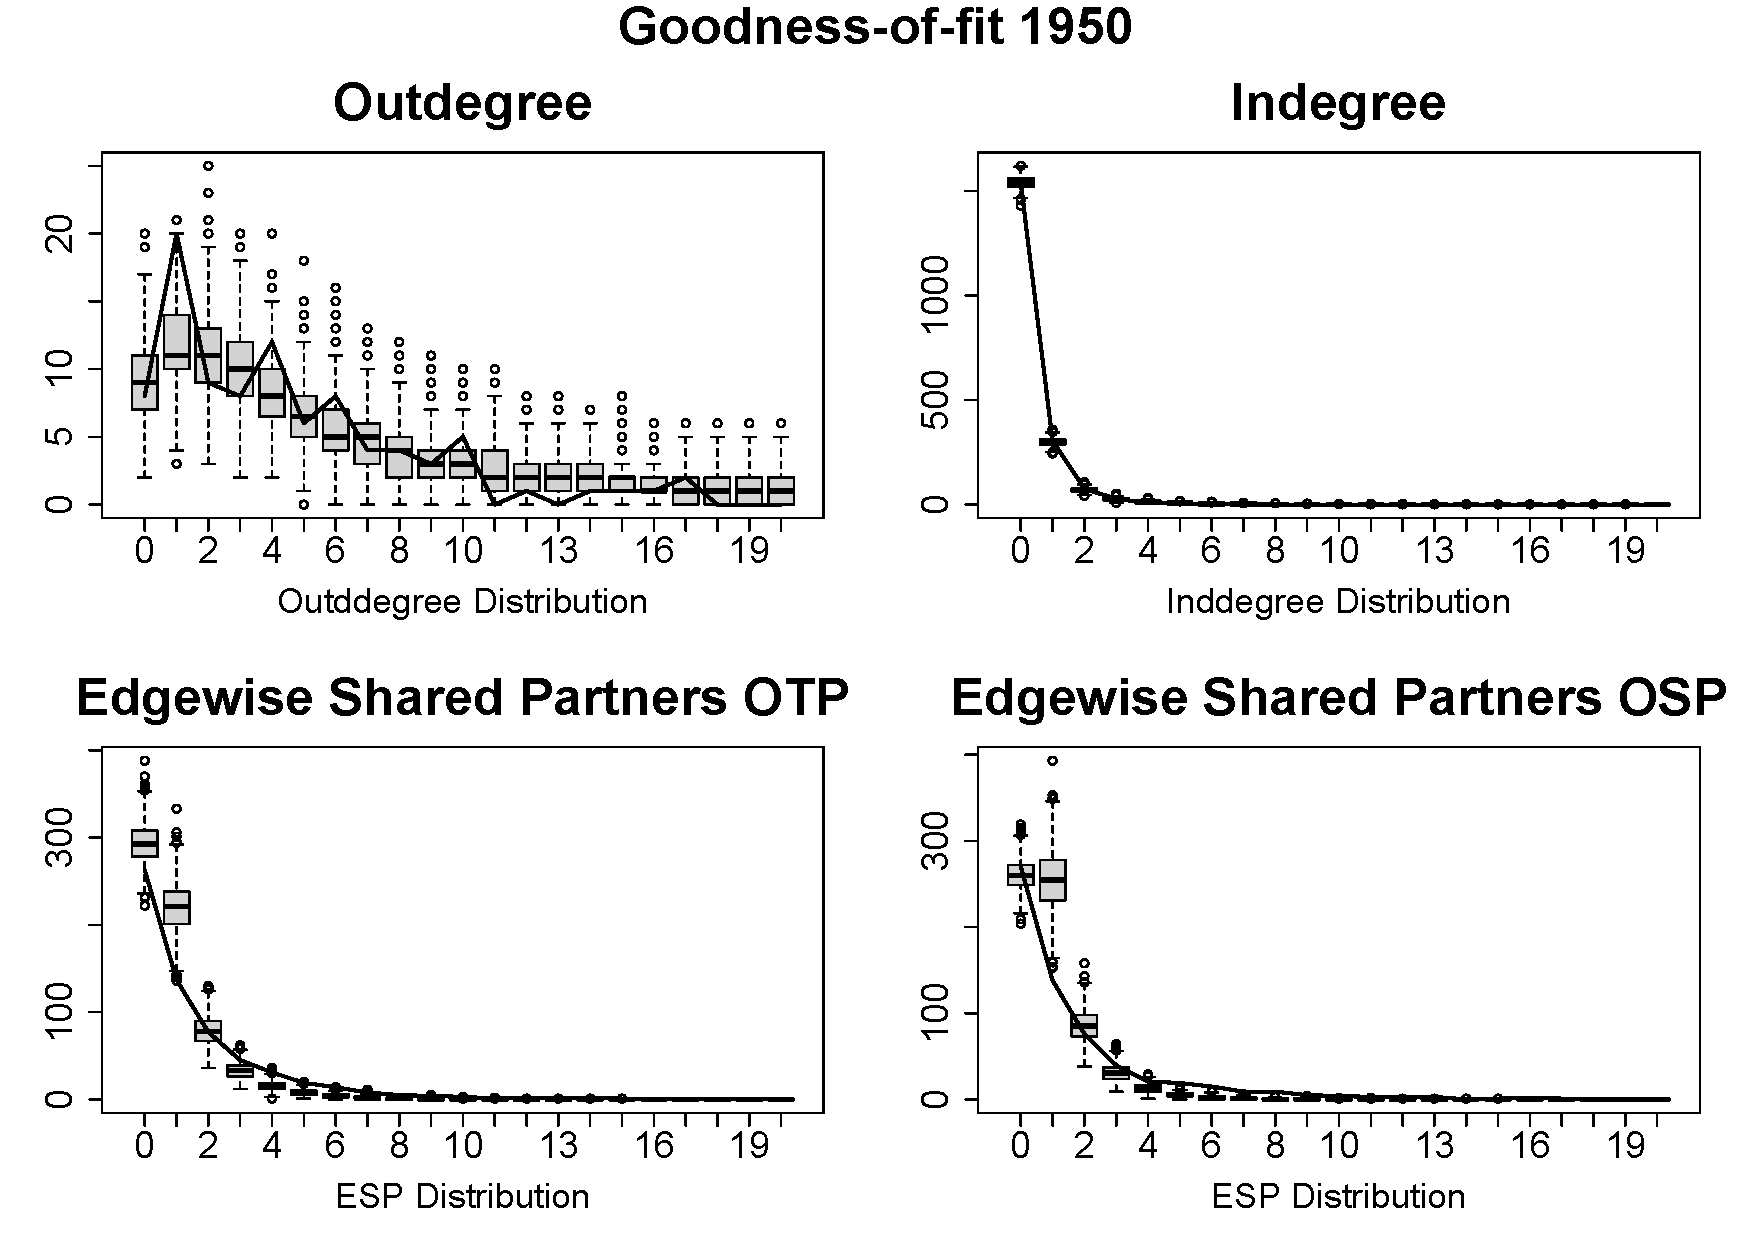
\includegraphics[width=13.8cm]{GOF_1950}\\
%\caption{Goodness-of-fit diagnostic for the 1950 network.}
% \label{GOF_1950}
\vspace{1cm}
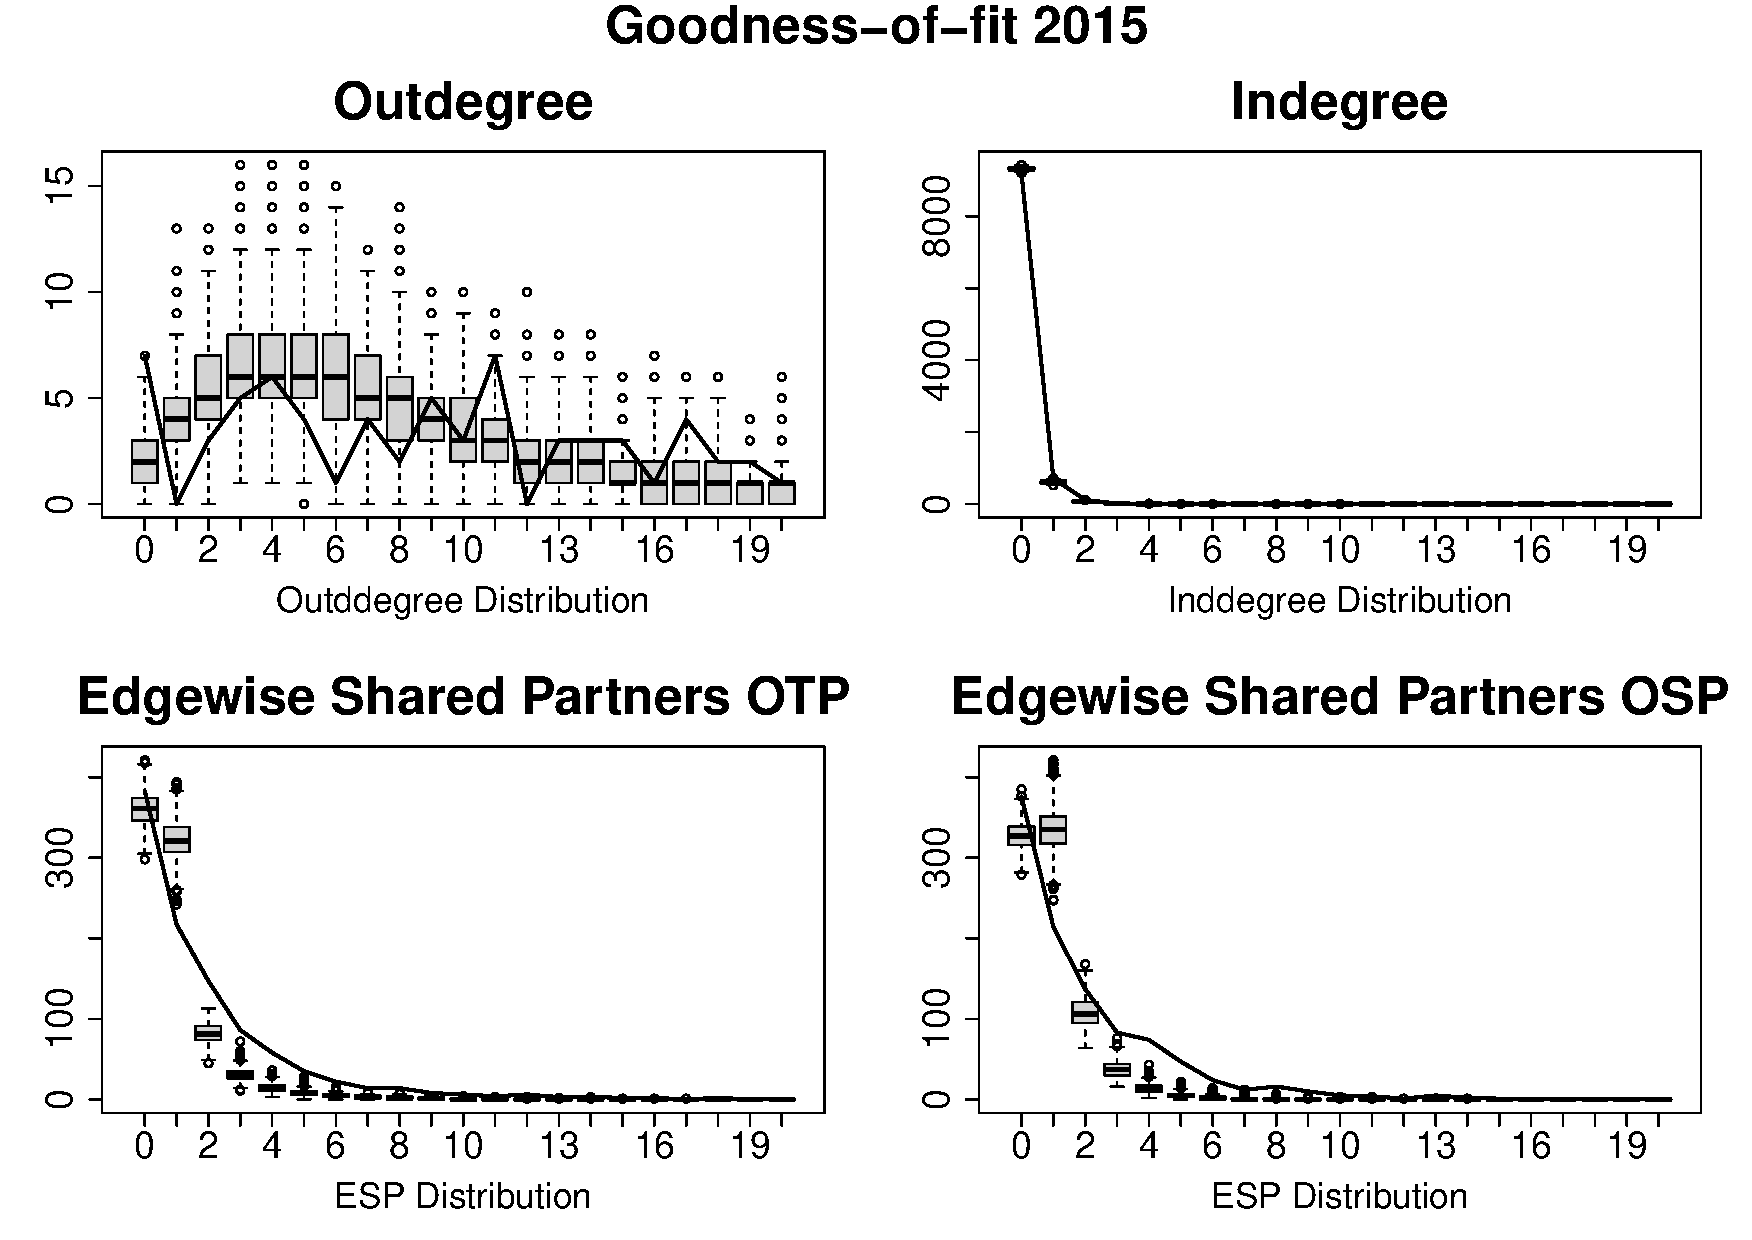
\includegraphics[width=13.8cm]{GOF_2015}
\vspace{0.1cm}
\caption{Goodness-of-fit diagnostic for the 1950 network (top) and the 2015 network (bottom).}
 \label{GOF}
\vspace{-.25cm}
\end{center}
\end{figure} 


\section{Checking for Model Degeneracy}

A common challenge when fitting ERGMs is model degeneracy. Model degeneracy occurs when the probability distribution defined by the parameter vector does not predominantly yield networks with similar statistics as the observed network. Generally, model degeneracy results in simulated networks with no ties or all possible ties. In a non-degenerate model the statistics of the networks that were simulated from the probability distribution defined by the MCMLE fall in the proximity of the observed network's statistics. Figures \ref{mcmcdiagnostics_1950} and \ref{mcmcdiagnostics_2015} depict trace and density plots for the dependence terms in the 1950 and 2015 term citation network. The histograms on the left visualize a statistic's density from $1000$ simulated networks, while the right side shows the statistic's trace plot of the same $1000$ networks. The solid black line indicates the statistic's value in the actual citation network. Both figures indicate that this model is non-degenerate and that the simulated network's statistics fall almost evenly around the observed statistic. The density and trace plots for the ERGM of the terms not depicted provide similar results.

\bibliography{bib} 
\bibliographystyle{apsr}

\begin{figure}[H]
 \begin{center}
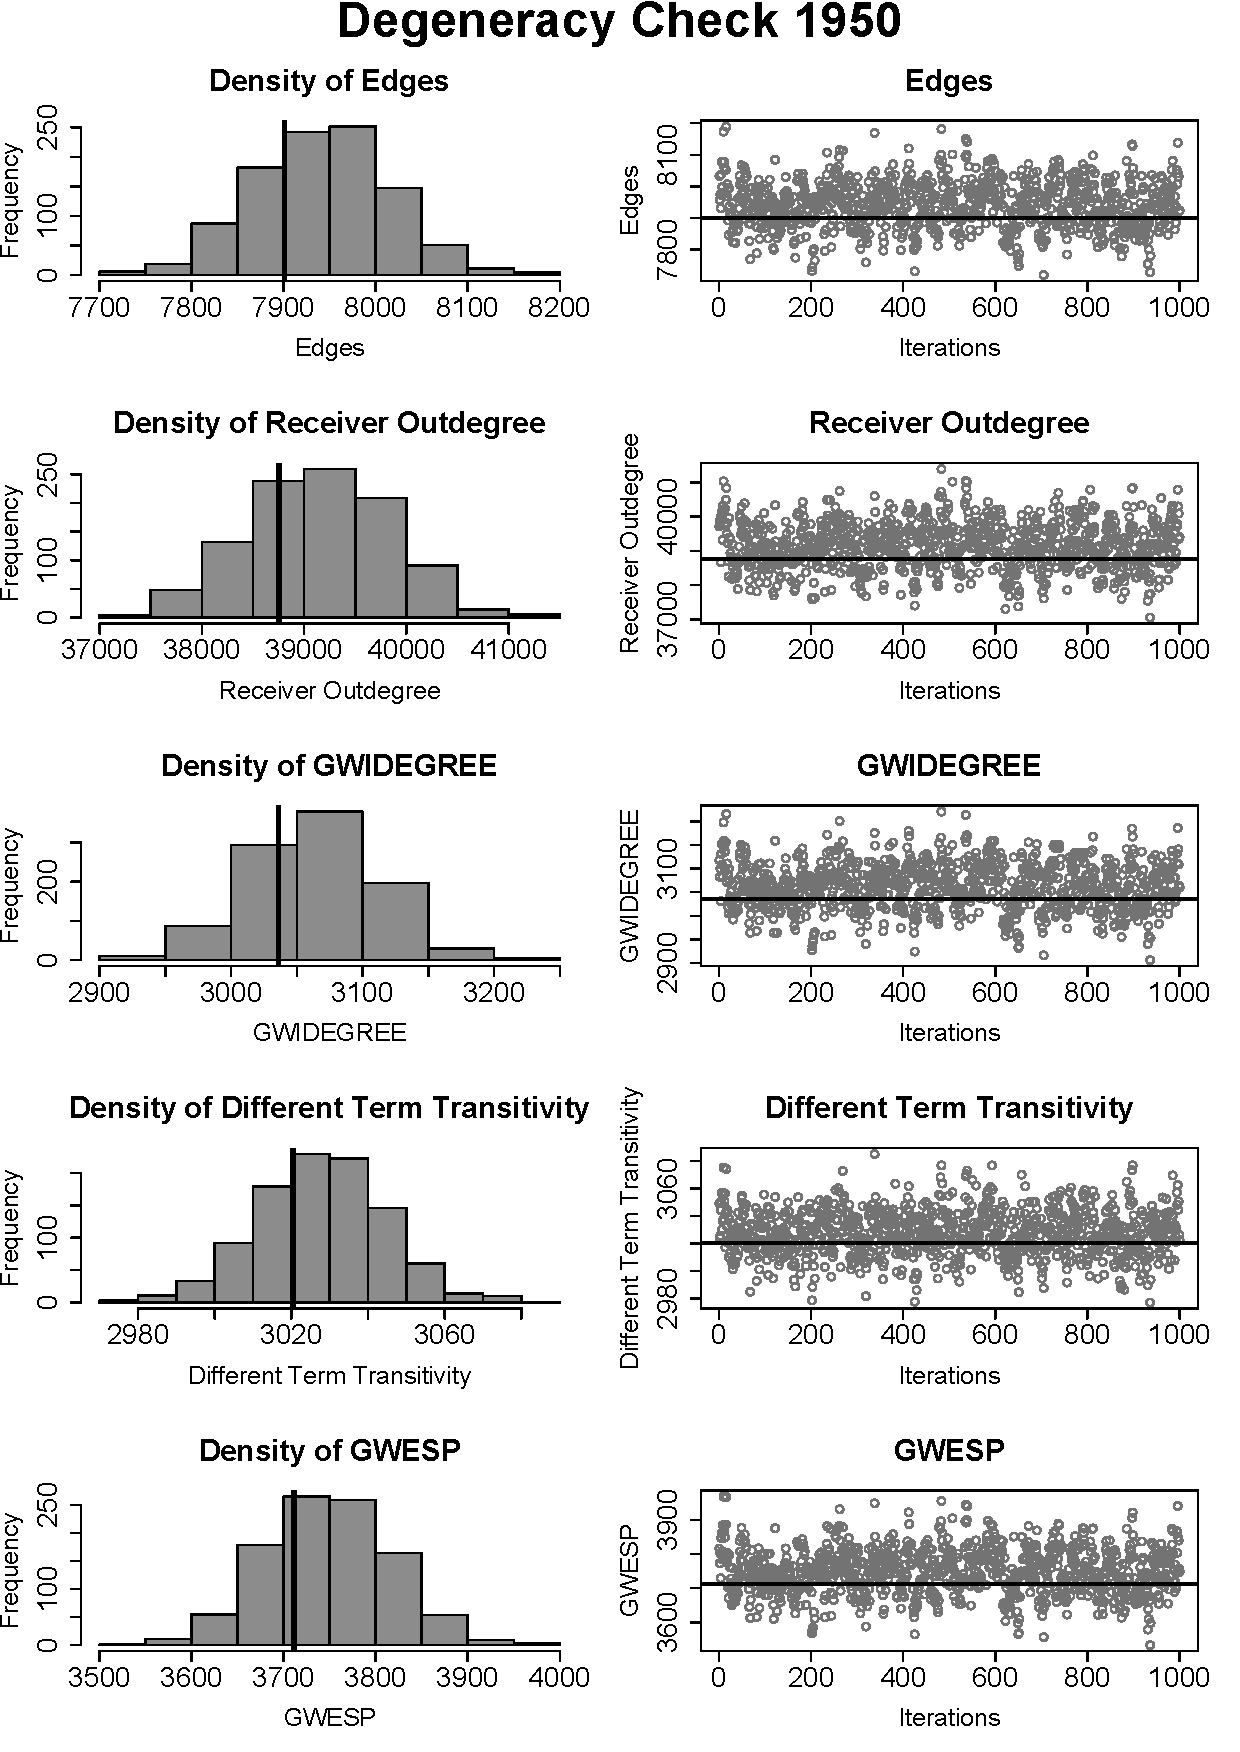
\includegraphics[width=14.5cm]{Deg_1950}
\caption{Density and trace plots for the dependency terms of the 1950 term citation network.}
 \label{mcmcdiagnostics_1950}
\vspace{-.25cm}
\end{center}
\end{figure} 


 \begin{figure}[H]
 \begin{center}
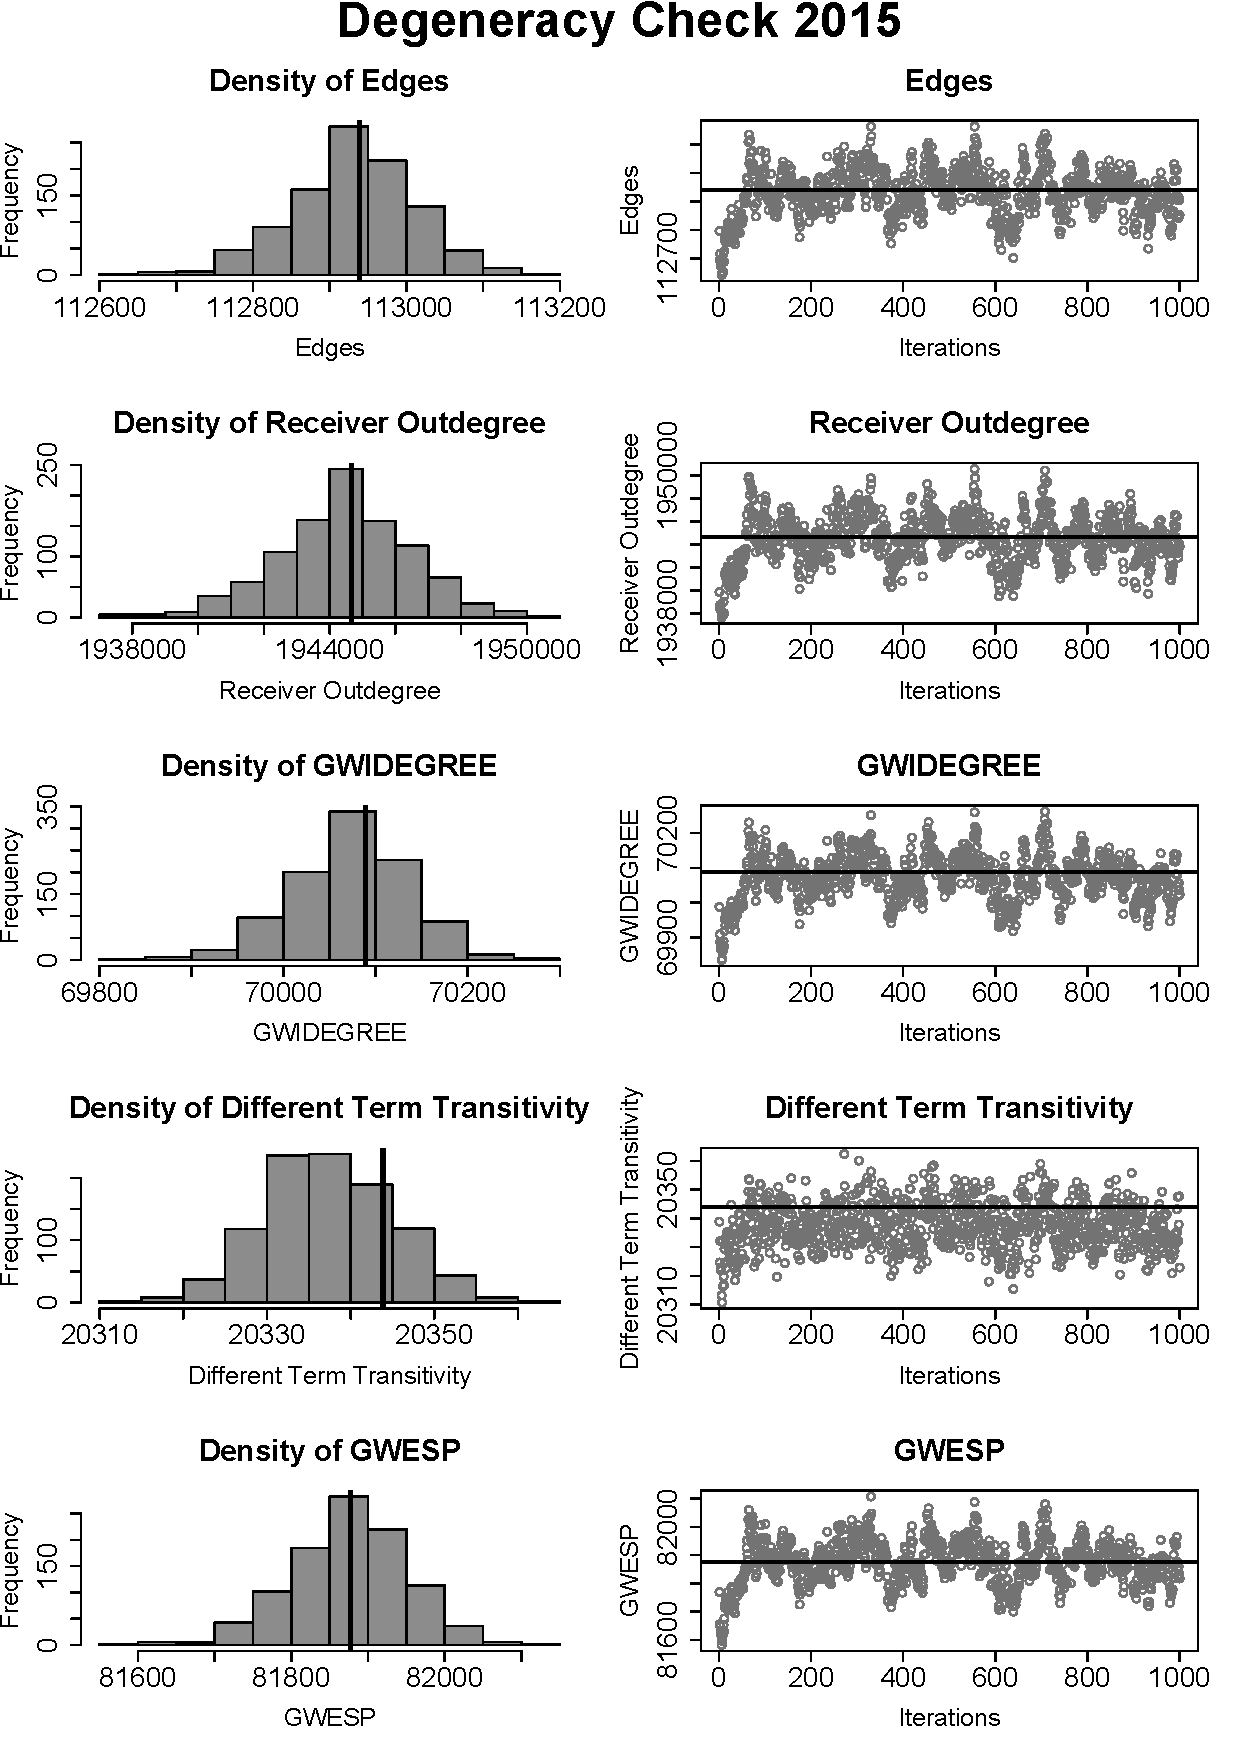
\includegraphics[width=14.5cm]{Deg_2015}
\caption{Density and trace plots for the dependency terms of the 2015 term citation network.}
 \label{mcmcdiagnostics_2015}
\vspace{-.25cm}
\end{center}
\end{figure} 





\end{document}




















